\section{How It Works}

\begin{frame}[fragile]{Standardized Prompt History Format - Part 1}
  \begin{block}{Example: .prompts/feature-auth.yaml - Metadata}
    \begin{lstlisting}[basicstyle=\ttfamily\small]
version: 1.0
metadata:
  created: 2025-10-09T10:30:00Z
  ai_tool: claude-code
  ai_version: sonnet-4.5
  author: developer@redhat.com
  repository: https://github.com/example/project
  commit: a1b2c3d4e5f6g7h8i9j0
\end{lstlisting}
  \end{block}

  \begin{block}{Key Metadata Fields}
    \begin{itemize}
      \item \textbf{version}: Schema version for compatibility
      \item \textbf{ai\_tool/ai\_version}: Specific AI model used
      \item \textbf{repository}: Git repository URL
      \item \textbf{commit}: Git hash linking prompts to code version
    \end{itemize}
  \end{block}
\end{frame}

\begin{frame}[fragile]{Standardized Prompt History Format - Part 2}
  \begin{block}{Example: .prompts/feature-auth.yaml - Prompt History}
    \begin{lstlisting}[basicstyle=\ttfamily\tiny]
prompts:
  - id: 1
    timestamp: 2025-10-09T10:30:00Z
    prompt: "Implement JWT authentication in Python using FastAPI"
    context:
      dependencies: ["fastapi", "pyjwt", "passlib"]
      requirements: "Python 3.11+, async support"
    files_generated:
      - src/auth.py
      - tests/test_auth.py
    validation:
      tests_pass: true
      coverage: 85%

  - id: 2
    timestamp: 2025-10-09T10:35:00Z
    prompt: "Add refresh token support to the auth module"
    context:
      based_on_prompt: 1
      security_considerations: "Store refresh tokens securely"
    files_modified:
      - src/auth.py
    files_generated:
      - src/refresh_tokens.py
    validation:
      tests_pass: true
\end{lstlisting}
  \end{block}
\end{frame}

\begin{frame}{Technical Components - Schema Structure}
  \begin{block}{Schema Structure}
    \begin{itemize}
      \item \textbf{Metadata}: Tool version, timestamps, git commit linkage
      \item \textbf{Context}: Dependencies, environment requirements, security notes
      \item \textbf{Lineage}: Track prompt chains and iterations
      \item \textbf{Validation}: Test results, coverage, quality metrics
    \end{itemize}
  \end{block}

  \begin{block}{File Organization}
    \begin{itemize}
      \item \texttt{.prompts/} directory in repository root
      \item One YAML file per feature/session
      \item Linked to commits via git hash
      \item Indexed by tags and keywords for search
    \end{itemize}
  \end{block}
\end{frame}

\begin{frame}{Technical Components - Capture Mechanisms}
  \begin{block}{Capture Mechanisms}
    \begin{itemize}
      \item \textbf{API Integration}: Hook into AI tool APIs (Claude, Gemini, etc.)
      \item \textbf{MCP Server Integration}
        \begin{itemize}
          \scriptsize
          \item Model Context Protocol server for standardized AI communication
          \item Intercepts prompts, responses, and tool calls
          \item Captures complete conversation context and history
          \item Enables bi-directional prompt flow (capture and replay)
        \end{itemize}
      \item \textbf{Git Hooks}: Automatic capture on commit/push
      \item \textbf{Manual Logging}: CLI tool for session recording
      \item \textbf{IDE Plugins}: Real-time capture in development environment
    \end{itemize}
  \end{block}

  \begin{block}{Benefits of Multiple Capture Methods}
    \begin{itemize}
      \item Flexibility for different workflows
      \item Fallback options if one method unavailable
      \item Integration with existing development tools
    \end{itemize}
  \end{block}
\end{frame}

\begin{frame}{Capture Mechanisms - Sequence Diagram}
  \begin{center}
    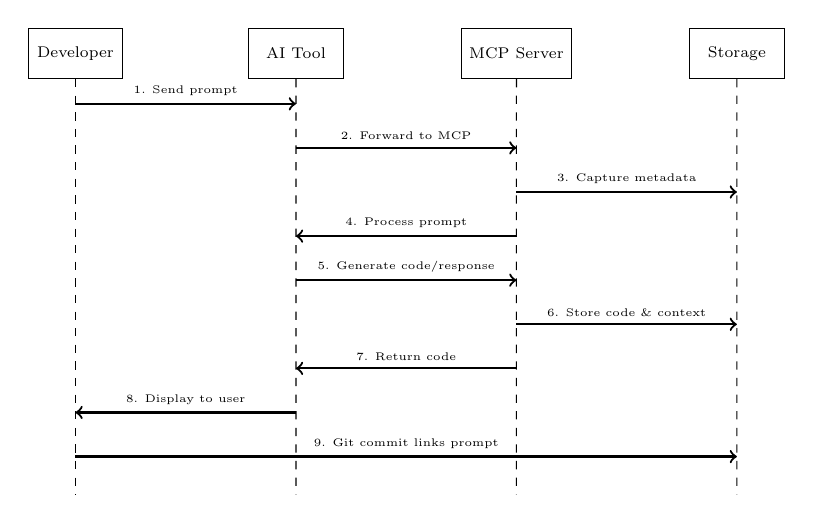
\begin{tikzpicture}[scale=0.8, every node/.style={scale=0.8}]
      % Actors
      \node[draw, rectangle, minimum width=1.5cm, minimum height=0.8cm] (dev) at (0,0) {\scriptsize Developer};
      \node[draw, rectangle, minimum width=1.5cm, minimum height=0.8cm] (ai) at (3.5,0) {\scriptsize AI Tool};
      \node[draw, rectangle, minimum width=1.5cm, minimum height=0.8cm] (mcp) at (7,0) {\scriptsize MCP Server};
      \node[draw, rectangle, minimum width=1.5cm, minimum height=0.8cm] (storage) at (10.5,0) {\scriptsize Storage};

      % Lifelines
      \draw[dashed] (dev) -- (0,-7);
      \draw[dashed] (ai) -- (3.5,-7);
      \draw[dashed] (mcp) -- (7,-7);
      \draw[dashed] (storage) -- (10.5,-7);

      % Interactions
      \draw[->,thick] (0,-0.8) -- node[above,sloped,pos=0.5] {\tiny 1. Send prompt} (3.5,-0.8);
      \draw[->,thick] (3.5,-1.5) -- node[above,sloped,pos=0.5] {\tiny 2. Forward to MCP} (7,-1.5);
      \draw[->,thick] (7,-2.2) -- node[above,sloped,pos=0.5] {\tiny 3. Capture metadata} (10.5,-2.2);
      \draw[->,thick] (7,-2.9) -- node[above,sloped,pos=0.5] {\tiny 4. Process prompt} (3.5,-2.9);
      \draw[->,thick] (3.5,-3.6) -- node[above,sloped,pos=0.5] {\tiny 5. Generate code/response} (7,-3.6);
      \draw[->,thick] (7,-4.3) -- node[above,sloped,pos=0.5] {\tiny 6. Store code \& context} (10.5,-4.3);
      \draw[->,thick] (7,-5.0) -- node[above,sloped,pos=0.5] {\tiny 7. Return code} (3.5,-5.0);
      \draw[->,thick] (3.5,-5.7) -- node[above,sloped,pos=0.5] {\tiny 8. Display to user} (0,-5.7);
      \draw[->,thick] (0,-6.4) -- node[above,sloped,pos=0.5] {\tiny 9. Git commit links prompt} (10.5,-6.4);
    \end{tikzpicture}
  \end{center}
\end{frame}
